\subsection{Training Strategy: Two-phase Training and Tax Curricula}
\label{sec:trainingstrategy}
As discussed in Section \ref{sect:innerouterrl}, the joint optimization problem posed by the inner-outer RL approach can lead to instability during learning.
One source of instability is that high tax rates cause large income penalties  during training, even for actions that might be optimal under low tax rates. Effective agent behaviors can be hard to learn due to this kind of noisy  feedback from an unconstrained, suboptimal planner  that generates random tax rates. We have found this to be especially problematic in the initial  phases of learning.

To stabilize learning we use a {\em two-phase training approach}.
In the first phase, we train a collection of agent models for a set of random seeds and without any taxes applied (the free-market scenario). This results in a set of agent models (one for each random seed) that are well adapted to the general game dynamics.

In phase two, we resume training, but with one of the studied tax models active.
In the case of the AI Economist, we also allow the planner to continue to adapt, along with  continued agent learning.
To avoid unstable learning dynamics created by the sudden introduction of taxes, we impose an {\em annealing schedule} over the early portion of phase two, during which a maximum limit on the allowable, marginal tax rates is linearly annealed from 10\% to 100\%.

Furthermore, we find that  {\em  entropy regularization} of the planner policy is necessary to achieve good outcomes in the face of these complex, joint learning dynamics.
Entropy regularization adds the policy's entropy as an additional, weighted term in the policy gradient objective, and is defined as
\eq{ \texttt{entropy}(\policy) = -\E_{\ac\sim\policy(.|\st)}\brcksq{\log\policy(\ac | \st)}.}

The use of this entropy term promotes  policies that explore more when used together with on-policy learning, which samples   trajectories according to the current policy $\policy$ \citep{williams1991function,mnih2016asynchronous}.

We perform experiments using the RLlib framework~ \citep{Liang2018_RLlib}.
We use {\em proximal policy gradients}~\citep{schulman2017proximal} and the Adam optimizer~ \citep{kingma_adam:_2014} to compute policy gradients.
Samples were collected from 60 environment replicas in parallel, using a sampling horizon of 200 timesteps between policy update iterations (a full episode consists of 1000 timesteps).
Trajectories were chunked into subsequences of length 50 for training the recurrent networks.
For more details, see the Appendix.
All experiments performed phase two training with 400 million samples, which we found to be sufficient for both agent and planner models to converge to stable policies.
The annealing schedule allows the maximum  marginal tax rate to reach 100\% by 54 million samples.
\begin{figure}[t!]
  \begin{small}
    \begin{center}
    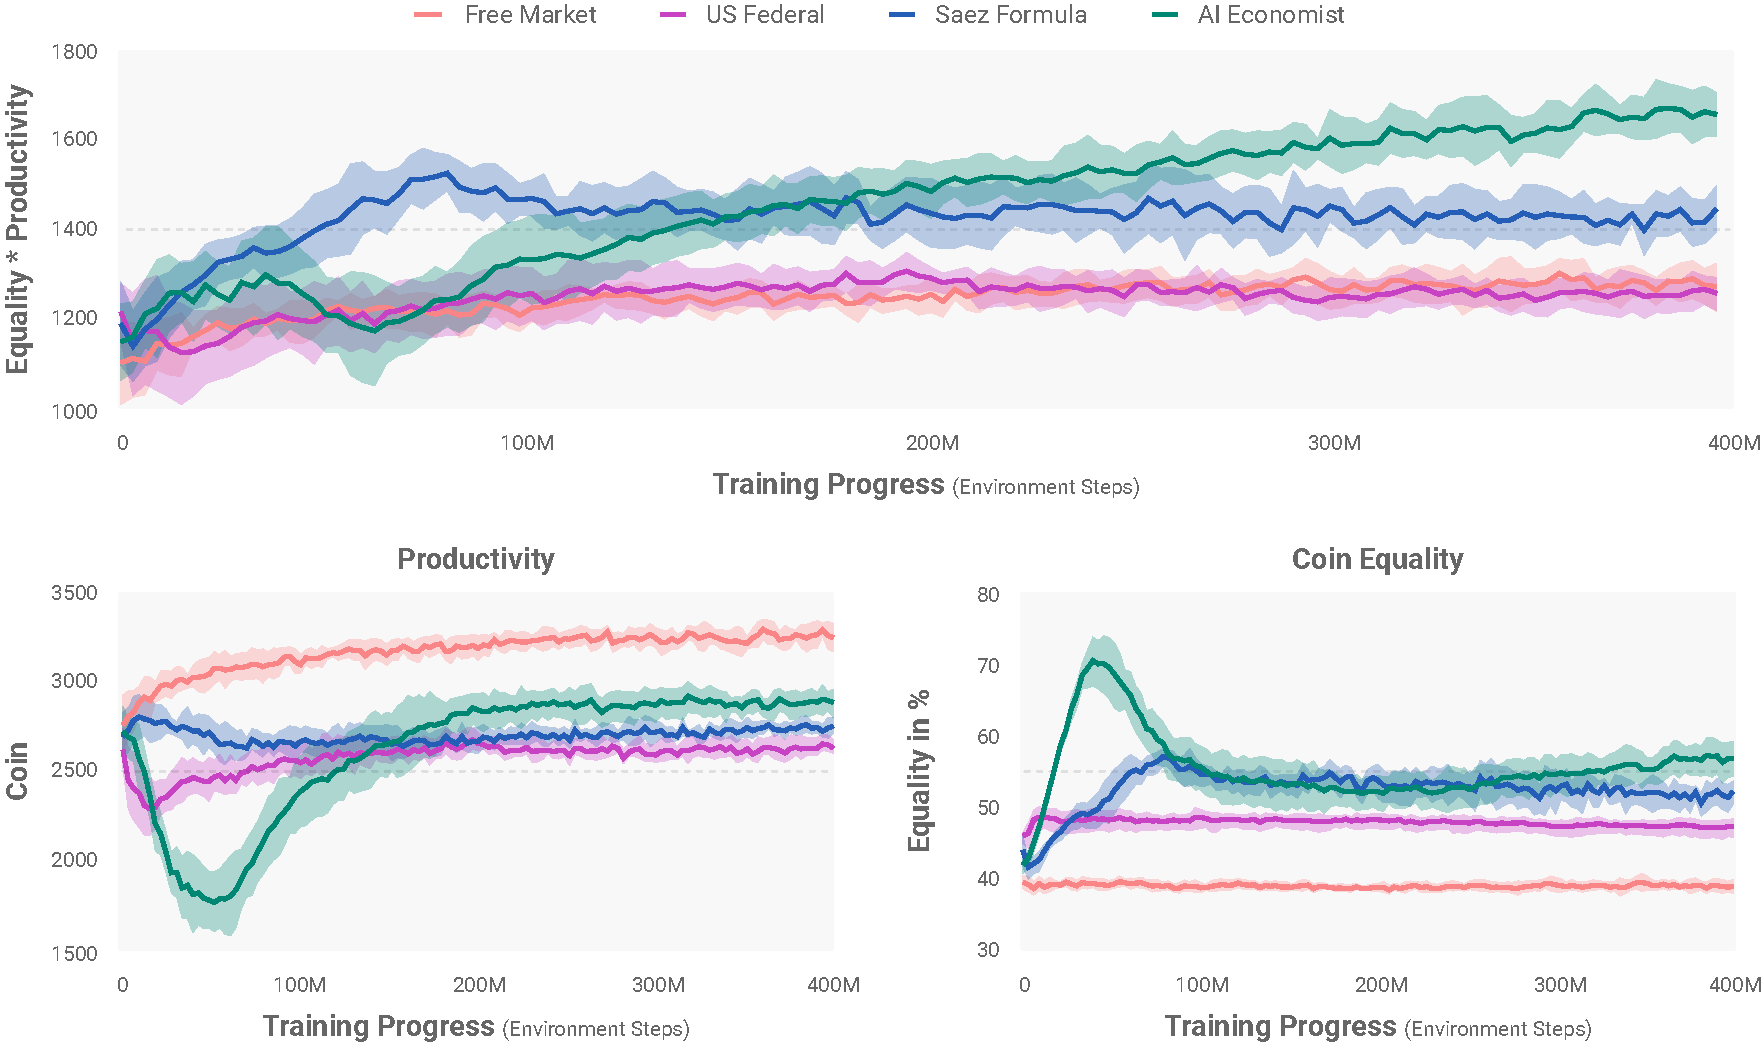
\includegraphics[width=0.95\textwidth]{figures/postprocessed/training-curves_postprocessed.pdf}
    \end{center}
    \caption{Empirical training progress for all models. The AI Economist (Green) achieves significantly better social outcomes than the baseline models. All baseline models have converged.}
    \label{fig:wandbcurves}
  \end{small}
\end{figure}


\subsection{Equality, Productivity, and Social Welfare Metrics}
\begin{figure}[t!]
  \begin{small}
    \begin{center}
    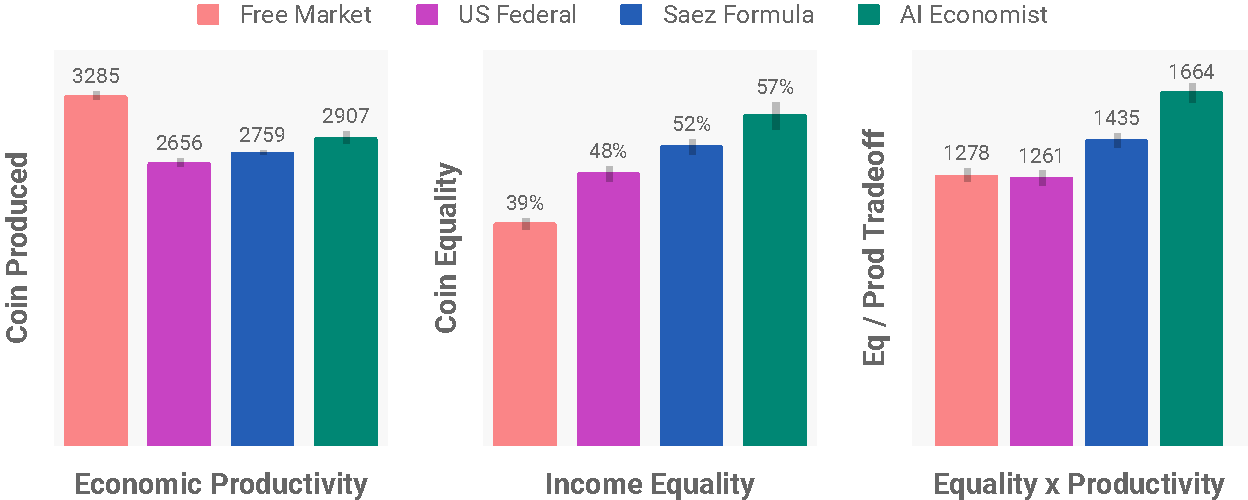
\includegraphics[width=0.617\textwidth]{figures/postprocessed/prod_eq_welfare_ai.pdf}
    \end{center}
    \caption{Comparison of overall economic outcomes (error bars show the variance during the final 20 million training steps, across 10 random seeds). The AI Economist achieves significantly better equality-productivity trade-offs compared to the baseline models. All baseline models have converged.}
    \label{fig:prod_eq_welfare_ai}
  \end{small}
\end{figure}
We compare economic outcomes under the AI Economist with the free market (no taxation or redistribution), a simulated US Federal tax schedule, and the tax policy that results from the Saez framework~\citep{saez_using_2001}.

For all four treatments we use reinforcement learning to optimize the behavior of the economic AI agents. The results are shown in Figure \ref{fig:prod_eq_welfare_ai}. Productivity (left panel, higher is better) measures the total amount of income generated within an episode (analogous to GDP). Taxation always results in a decrease of productivity when compared with the free market, but the loss in productivity is the smallest under the AI Economist. Income equality (middle panel, higher is better), which is defined as 1 - Gini index and computed at the end of an episode (higher Gini index means incomes are less equal), is highest under the AI Economist.
The product of equality and productivity (right panel, higher is better) measures the balance between equality and productivity. The AI Economist achieves a 16\% gain improvement over the next best model, which is the Saez model. The AI Economist also improves equality by 47\% compared to the free-market, at only an 11\% decrease in productivity.

As discussed in Section \ref{sec:opttax}, the challenge in setting taxes stems from the inherent trade-off between equality and productivity.  This can be  seen in the empirical results, where
redistribution  improves equality but at the cost of productivity.\footnote{We also find in our experiments that total redistribution (such that all workers have the same income after redistribution) yields perfectly equal but highly unproductive economies and very low equality-vs-productivity trade-offs.}
This property naturally emerges  in our simulations, by allowing agents to learn optimal responses to  taxes.

In summary, these results demonstrate (1) that our framework allows us to reproduce the central challenge considered in optimal taxation theory, the trade-off between equality and productivity, (2) that the severity of this trade-off depends on the choice of tax schedule, and (3) that RL can be used to optimize tax policies.

\subsection{Tax Schedules and Wealth Redistribution after Taxes and Subsidies}
\begin{figure}[t!]
  \begin{minipage}[t]{0.48\linewidth}
    \begin{small}
    \begin{center}
      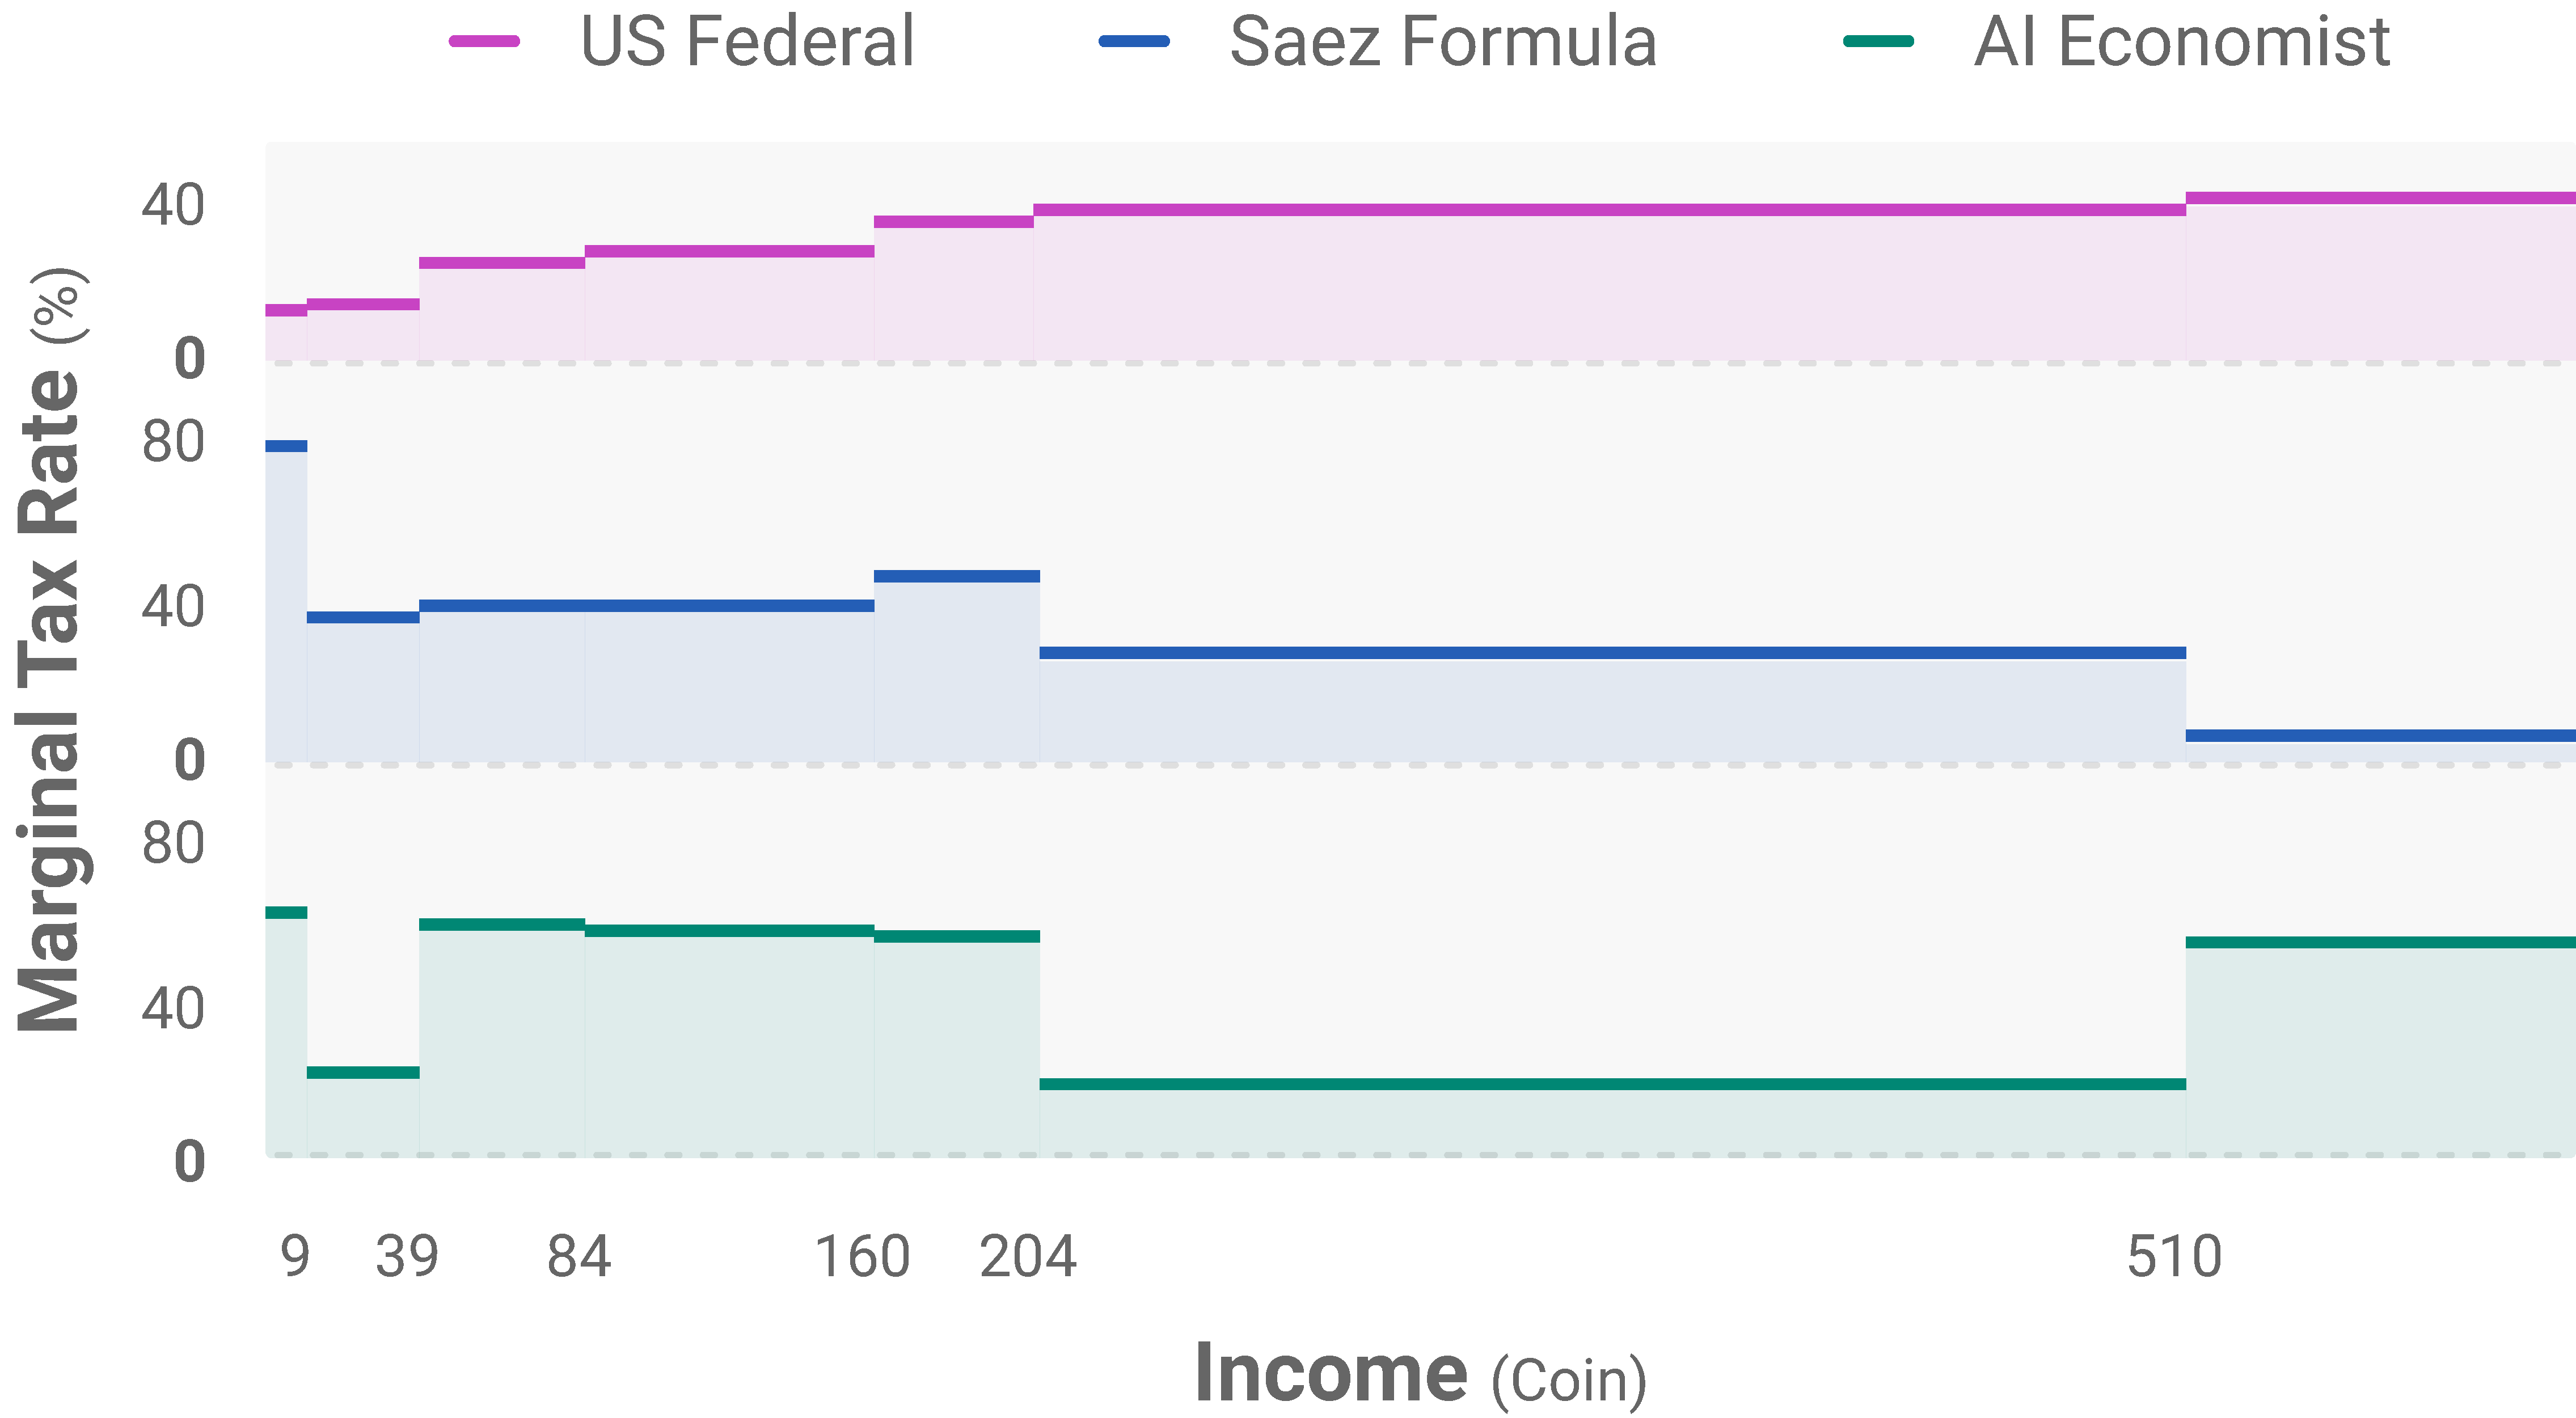
\includegraphics[width=\textwidth]{figures/postprocessed/marginal-rate-schedules.pdf}
    \end{center}
    \caption{Comparison of average tax rates per episode. Variances within the Saez and AI Economist schedules are not shown. On average, the AI Economist sets a  higher top tax rate than both of the US Federal and Saez tax schedules. The free-market collects zero taxes.
    }
    \label{fig:tax_rates_ai}
    \end{small}
  \end{minipage}
  \hspace{0.03\linewidth}
  \begin{minipage}[t]{0.48\linewidth}
    \begin{small}
    \begin{center}
      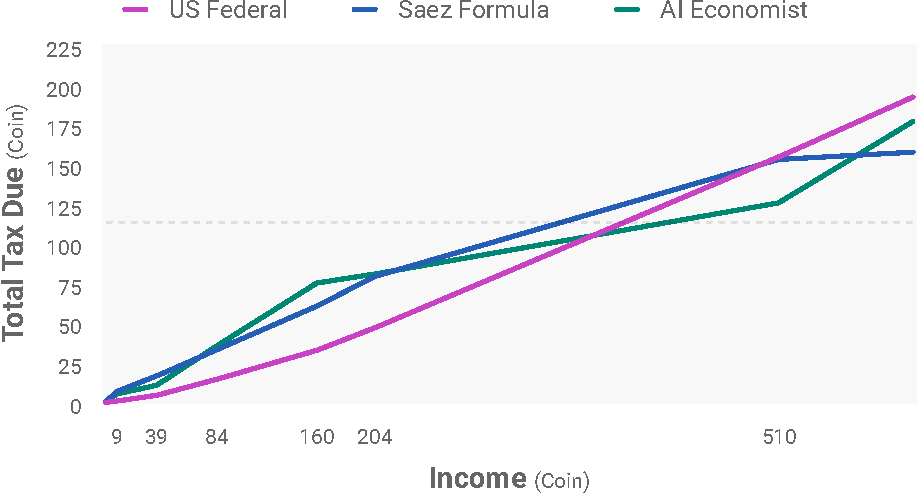
\includegraphics[width=\textwidth]{figures/postprocessed/dollar_taxes_ai_only.pdf}
    \end{center}
    \caption{The effective taxes payable as a function of income. The taxes grow faster under the Saez and AI Economist schedules than under the US Federal schedule. But this does not include the effect of subsidies that arise from this collection of taxes (in effect, lower incomes  receive net subsidies, see Figure \ref{fig:tax_impact_per_agent}).}
    \label{fig:effective_tax_ai}
    \end{small}
  \end{minipage}
\end{figure}
\begin{figure}[t!]
  \begin{small}
    \begin{center}
    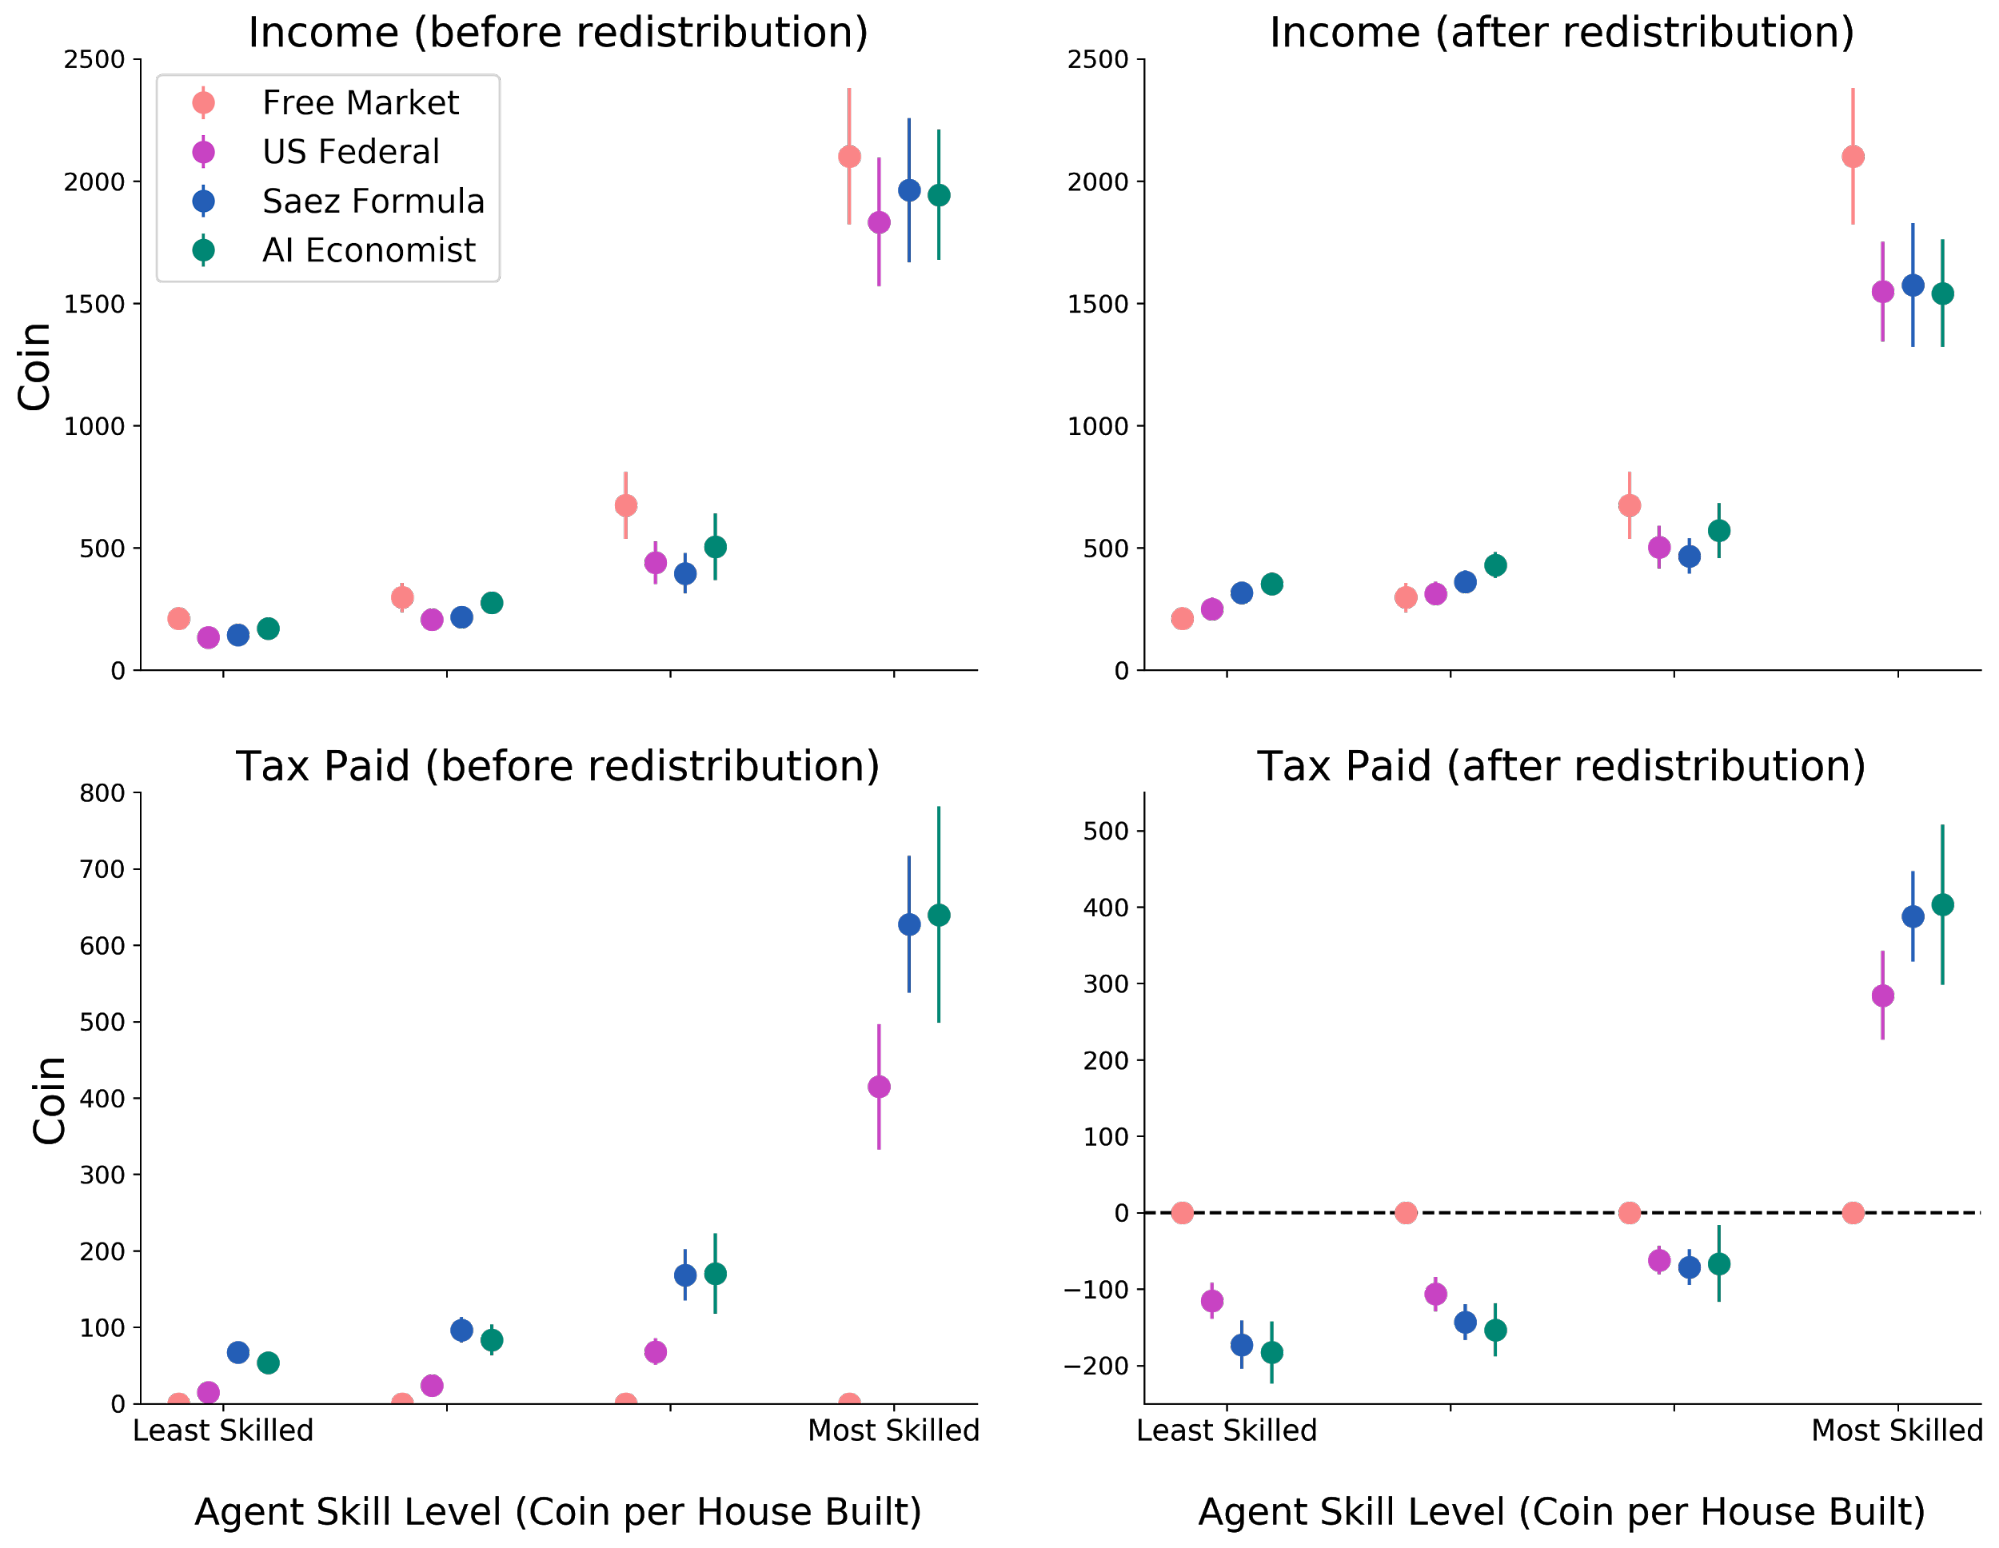
\includegraphics[width=0.8\textwidth]{figures/tax_impact_per_agent.png}
    \end{center}
    \caption{Agent-by-agent averages after sorting by skill. Income before redistribution (top-left) shows the average pre-tax income earned by each kind of agent. The amount of tax paid before distribution is shown in the bottom left. The amount of tax paid after redistribution is shown in the bottom right (the lower skill agents receive a net subsidy).   The income after redistribution (top-right) shows the net average coin per agent at the end of the episode (the lower-skilled agents have higher net income under the AI Economist’s tax scheme).}
    \label{fig:tax_impact_per_agent}
  \end{small}
\end{figure}
\paragraph{Comparing Tax Schedules.}
All tax models control the marginal tax rates applied to each of seven income brackets (see Figure \ref{fig:tax_rates_ai}, which illustrates the average bracket rate set by each model).
We set up the economic simulation such that the fraction of agent incomes per income bracket are in rough alignment with those in the US economy\footnote{Based on preliminary experiments with the US Federal tax policy.}.

The 2018 US Federal tax rates are progressive, with a marginal tax rate  that increases with higher  income. For the present setting, and with the social welfare objective that we adopt, the Saez tax framework mostly sets a regressive tax schedule, with a marginal tax rate that decreases with higher income. The AI Economist features a more idiosyncratic structure, with a blend of progressive and regressive tax schedules. In particular, it sets a higher top tax rate (on income above 510), a lower tax rate for incomes between 160 and 510, and both higher and lower tax rates on incomes below 160.
\paragraph{Effective Tax After Redistribution.}
The AI Economist's tax schedule provides higher subsidies to low income agents than the baselines. %
The  agents have different skill levels, and the learned behaviors, incomes, and amount of tax paid all depend heavily on skill. Figure \ref{fig:tax_impact_per_agent} presents the agent-by-agent averages after sorting by skill. Income before redistribution (top-left) shows the average pre-tax income earned by each kind of agent. Tax paid is shown in the bottom left. The effect of redistribution,  which equally divides collected taxes among the agents, is that the lower-skilled agents receive a net subsidy (bottom right). The income after redistribution shows the net average coin per agent at the end of the episode (top right). The lower-skilled agents have higher net income under the AI Economist than under the other models.


\paragraph{The Impact of Tax on Economic Activity.}
\begin{figure}[t!]
  \begin{small}
    \begin{center}
    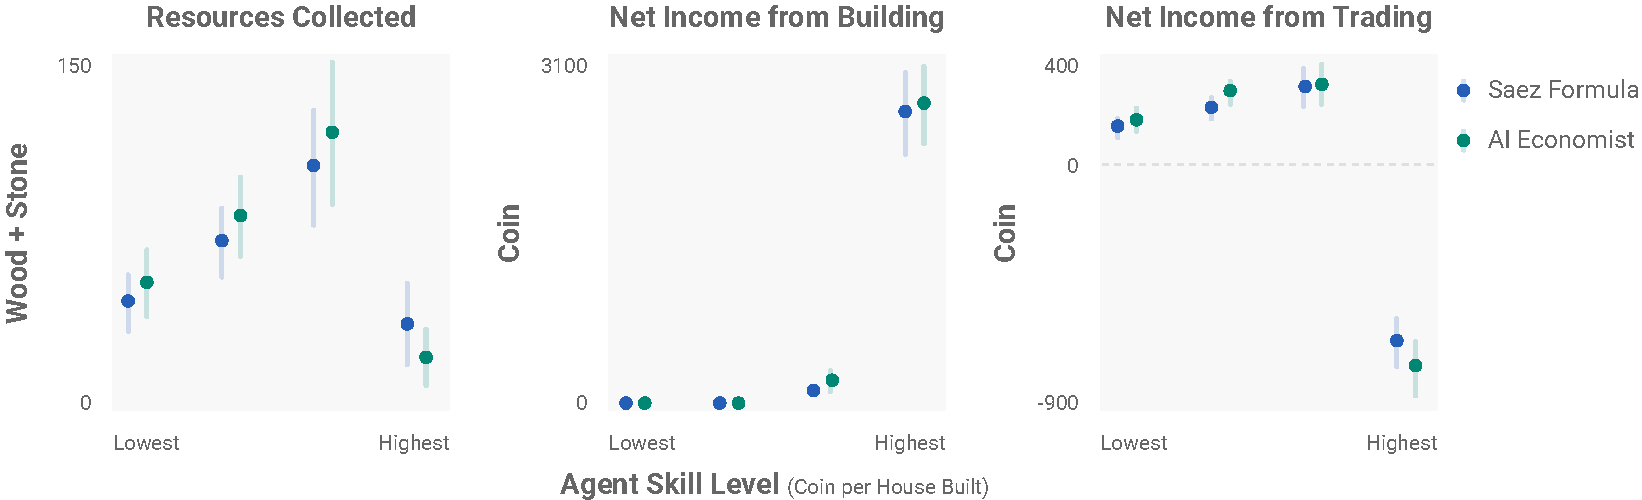
\includegraphics[width=0.9\textwidth]{figures/postprocessed/saez-aieconomist-comparison.pdf}
    \end{center}
    \caption{
    Comparing the impact of tax on economic activity for the Saez formula and the AI Economist.   Left: Average number of resources (both wood and stone) collected per episode for each of the four agents.
      Middle: Average (per episode) total income earned from building.
      Right: Average (per episode) total income earned from trading. Negative income means the agent spends more than it earned.
      Lines indicate the standard deviation.
    }
    \label{fig:saez-aieconomist-comparison}
  \end{small}
\end{figure}

To form a better understanding of how taxes set by the AI Economist improve over those set by the Saez formula, which provides the strongest baseline, we compare their respective impacts on the agents' economic activity (Figure \ref{fig:saez-aieconomist-comparison}).
In both cases, the low-income agents  choose to specialize as ``gatherer-and-seller” agents.
Interestingly, these agents collect fewer resources under the Saez policy, and the high-skilled ``buyer-and-builder” agent compensates by increasing its own resource collection (Left panel).
This de-specialization  contributes to the decreased income generated through building under the Saez taxes (Middle panel), with this decrease accounting for  weaker productivity.

Because the Saez formula leads to a more regressive tax structure than the AI Economist, the latter yields higher equality through \textit{mechanical} effects (i.e. stronger redistribution).
Interestingly, the AI Economist also improves equality through \textit{behavioral} effects.
Under the Saez scheme, the ``buyer-and-builder'' collects more resources directly from the environment, meaning it makes fewer purchases from the other agents. Trading  serves to redistribute the income achieved from building houses to the ``gatherer-and-seller'' agents, but, owing to the behavioral differences, this redistributive effect is stronger under the AI Economist (Right panel).
From this perspective, the tax scheme discovered by the AI Economist appears better adapted to the complex economic interactions that shape both equality and productivity.

\subsection{Tax-Gaming Strategies}
\begin{figure}[t!]
  \begin{small}
    \begin{center}
    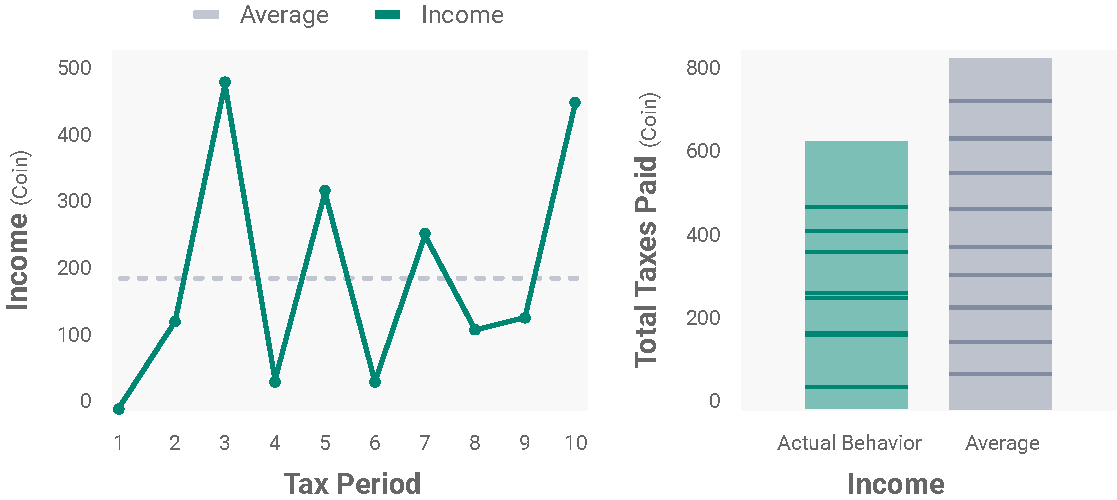
\includegraphics[width=0.7\textwidth]{figures/postprocessed/period-tax-example-improved.pdf}
    \end{center}
    \caption{Left: Income of the highest-skilled agent for each tax period in an example episode with the AI Economist (green line).  The dashed grey line shows the agent's average income. Right: Comparison of the total amount of tax the agent owed based on its actual  income (green) and the tax it would have owed if it reported its average income in each period (gray). Each box in the column denotes the tax obligation in a single period.
    }
    \label{fig:tax_episode}
  \end{small}
\end{figure}

Figure~\ref{fig:tax_episode} provides an example of the  income and taxes collected during an episode of the AI Economist environment, shown here after the tax policy has converged. Recall that each episode is divided into ten tax periods of equal length. At the start of each period, a new tax schedule is set by the AI Economist according to the new world state. Agents act in the environment,  earn income, and  taxes are collected at the end of the period according to the tax schedule and redistributed.


We see emergent tax gaming, where AI agents  learn to lower their average effective tax by alternating between earning high and low incomes in each period, rather than smoothing their income across  tax periods.
Figure~\ref{fig:tax_episode} (left) shows there is considerable variability in income earned from period to period, shown here for the highest skilled agent.  Figure~\ref{fig:tax_episode} (right)
 shows  the total amount of taxes paid given this behavior, together with the total taxes that would be paid if the  income had been smoothed across periods.

We see this kind of tax avoidance behavior in our experiments  for both the Saez and AI Economist models, which   feature lower top tax rates (regressive schedules), making it more tax-efficient to earn high incomes. This underscores the richness of the simulation-based learning framework. Moreover, the  AI Economist remains effective even in the face of this kind of strategic  behavior.